\documentclass{article}
\usepackage{amsmath}
\usepackage{hyperref}
\usepackage{bookmark}
\usepackage{float} 
\usepackage{graphicx}
\usepackage{makeidx}
\usepackage[letterpaper, total={7.5in, 10in}]{geometry}

\makeindex
\begin{document}
\title{Charges and Charging, and Coulomb's Law}
\author{Elias Xu}
\date{\today}
\maketitle
\setlength{\parindent}{0pt}

\section{Charging Introduction}

These are my notes on charges and charging for Physics!

\medskip

Charges are fundamental properties for particles, just like \textbf{masses} and \textbf{spins}.

\section{Fundamental Properties of Particles}

There are three particles that matter for charges and charging.

\begin{table}[h]
    \centering
    \begin{tabular}{|c|c|c|}
        \hline
        Particle & Charge (in \textit{e}) & Charge (in Coulombs (C)) \\
        \hline
        Proton   & 1\textit{e}            & $1.6 \times 10^{-19}$ C  \\
        Electron & - 1\textit{e}          & $-1.6 \times 10^{-19}$ C \\
        Neutron  & 1\textit{e}            & $1.6\times 10^{-19}$ C   \\
        \hline
    \end{tabular}
\end{table}

Charges are usually sent in multiples of elementary charge, usually through electrons (because if you remove protons, the atoms themselves change).

\medskip
\textbf{Note}: Elementary charges are elementary because they are the smallest stable charge. You can get quarks (with fractions of elementary charges), but will reform to these particles.

\section{Sending and Receiving Charge}

There are three methods for sending and recieving charge:

\begin{itemize}
    \item Friction
    \item Conduction
    \item Induction
\end{itemize}

\subsection{Friction}

\begin{figure}[H]
    \centering
    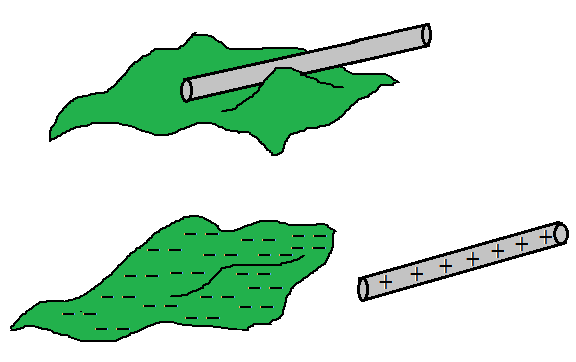
\includegraphics[width=0.2\textwidth]{figures/friction.png}
    \caption{Example of Friction}
\end{figure}

When two objects rub with each other, the object with higher affinity will \textbf{take} electrons from the other.

Usually, if you have two of the same object rub the same way, the objects have the same charge.

\subsection{Conduction}

\begin{figure}[H]
    \centering
    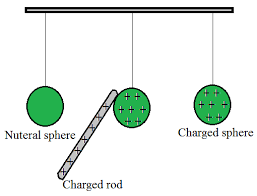
\includegraphics[width=0.2\textwidth]{figures/conduction.png}
    \caption{Example of Conduction}
\end{figure}

When two conductors (all objects are conductors in the end, if you try hard enough). If objects are identifical, their charge will even out. Elsewise, they will just equalize. If I remember correctly, applying the "same" friction will cause the same charge result.  \\~\\
\textbf{Note}: These conductors equalize to minimize the system's \emph{kinetic energy}.

\subsection{Induction}

\begin{figure}[H]
    \centering
    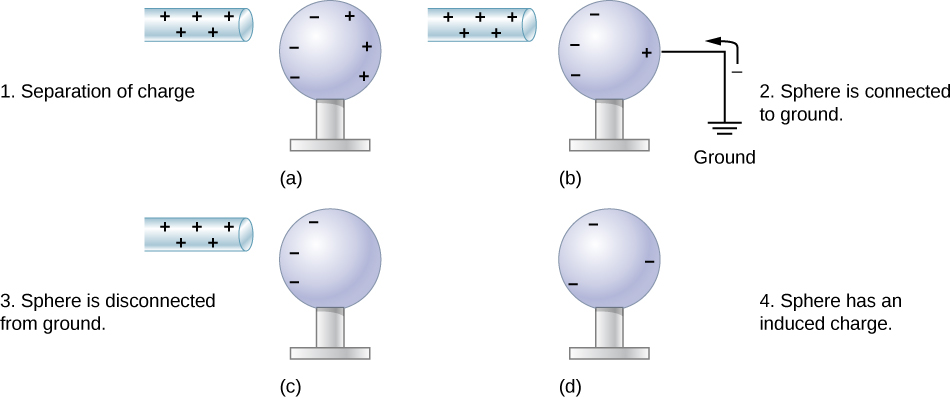
\includegraphics[width=0.5\textwidth]{figures/induction.jpg}
    \caption{Example of Induction}
\end{figure}

A charge can change through proximity to an object. To equalize the charge afterwards, you can just tap the two objects together (if I remember correctly).

\subsection{Note: Polarized Neutral}

\begin{figure}[H]
    \centering
    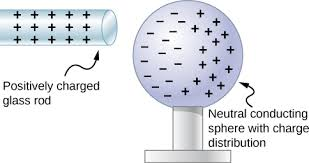
\includegraphics[width=0.2\textwidth]{figures/neutral_polarization.jpeg}
    \caption{Example of a polarized neutral}
\end{figure}

A neutral object can be polarized through having the charged object attract the opposite charge of a neutral object, causing attraction through the distance.

\subsection{Note: Question Stuff}

The question worksheet was \textit{Electric Charge and Methods of Charging}, and the only weird thing was question 4. To solve, just do
\[
    \frac{1.5 \, \text{m} \times \left(6.023 \times 10^{23} \, \text{particles} \, \text{per} \, \text{m}\right)}{1 \times 10^6 \, \text{particles per e}} \times \frac{1.6 \times 10^{-19} \, \text{C}}{e} = 0.144 \, \text{C}
\]
$6.023 \times 10^{23}$ is Avogadro's (Avocado's) number, which is equal to the number of particles per mole. One just has to divide by that the number of particles before one is charged, and then to convert elementary charges to coulombs.


\section{Coulomb's Law}

Coulomb's Law is related to how two charged particles are attacted to each other.

\subsection{Coulombs's Law from Regents}

$$F_e = \frac{k q_1 q_2 }{ R^2}$$

Problems with this formula:

\begin{itemize}
    \item $k$ assumes a vacuum
    \item $q_1 \text{ , } q_2$ are point particles
    \item One has to assume one object is stationary
\end{itemize}

\subsection{Building from Coulomb's Law for Physics C}

\begin{enumerate}
    \item We don't want to use $k$ anymore. Instead we use $\frac{1}{4 \pi \epsilon}$. $\epsilon$ represents the permittivity of a material \footnote{the ability of a particle to hold energy at a specific field without breaking down}. For vacuums, the permittivity, or $\epsilon_0$, is equal to $8.85 \times 10 ^ {-12} \frac{\text{C}^2}{\text{Nm}^2}$
    \item To fix the fact that that $q_1 \text{ and } q_2$ must be point particles, one will have to integrate over $\delta q$, or change in charge, to find the total charge, and integrate over $\delta F$. to find the force.
\end{enumerate}

Putting everything together, we have the new formula:
$$\boxed{ \vec{F_e} = \frac{1}{4 \pi \epsilon} \frac{q_1 q_2}{R^2} \hat {r}}$$ \\
where $\hat {r}$ is vector pointing to the other charge, making it so that when the equation positive, the resultant vector is pointed away from the other particle. Remember, $\boxed{\epsilon_0 = 8.85 \times 10 ^ {-12} \frac{\text{C}^2}{\text{Nm}^2}}$ [this is also on the reference table]

\section{Electrical Fields}
\begin{figure}[H]
    \centering
    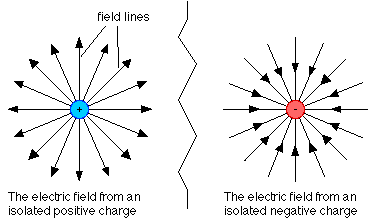
\includegraphics[width=0.2\textwidth]{figures/physicsfields1.png}
    \caption{Examples of a Electrical Field}
\end{figure}
The formula for calculating a electirc field, which is the force on the probe charge divided by the charge:
$$\vec{E}(r) = \frac{\vec{F}_0(r, q_0)}{q_0} = \frac{\frac{1}{4\pi\epsilon_0} \frac{Qq_0}{r^2}}{q_0} = \boxed{\frac{1}{4\pi\epsilon_0} \frac{Q}{r^2}\hat{r} \frac{\text{N}}{\text{C}}}$$

\textbf{NOTE}: Always assume that the satellite particle is positive. \\~\\

\textbf{Example} \\
The figure below shows a proton $p$ and an electron $e$ on an x-axis. What is the direction of field due to the electron at points S and R, and then the net charge.
\begin{figure}[H]
    \centering
    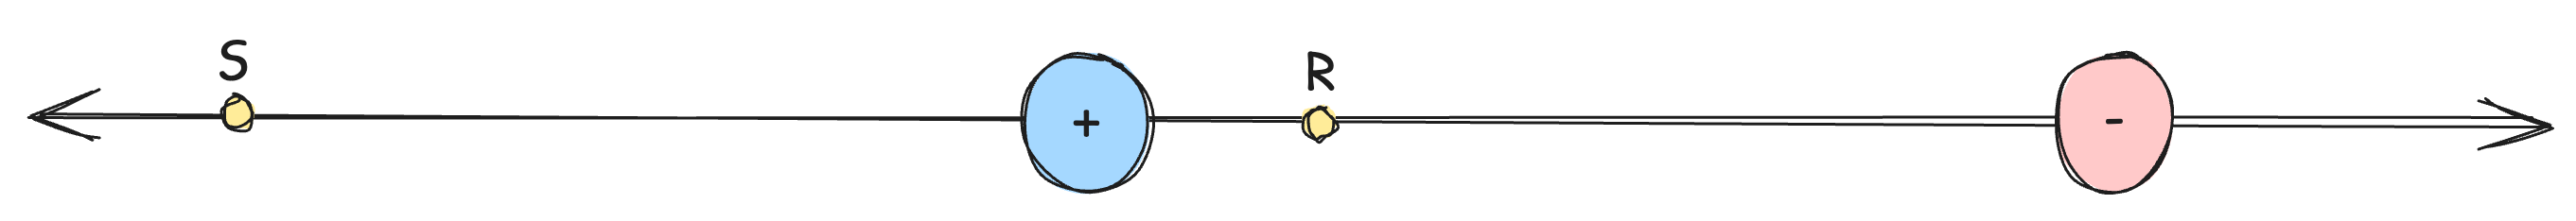
\includegraphics[width=0.9\textwidth]{figures/ElectricFieldExampleProblem.png}
\end{figure}
\begin{itemize}
    \item The electron's field on S is towards the electron in a rightward direction, and at R is towards the electron in a left direction
    \item The net field at S is a lesser (lesser magnitude) arrow towards the right, and at R its a larger arrow (greater magnitude) to the left.
\end{itemize}

\subsection{Calculating the Electrical Charge of Non-Point Particles}
If we have a long thin rod, we have a few methods to try to integrate and find the field:
\begin{itemize}
    \item You can integrate (\textbf{DRAWBACKS}: Both wierd directionally and changes with the charge too, not always ideal)
    \item Chickening out and using a $\infty$ lengthed rod, or use \textbf{Gauss' Law} (ohhhhh...)
\end{itemize}

\section{Calculating Continuous Charge Distributions for a Ring}
Reminder: It's arbitrarily difficult to calculate the charge of a continious shape. Therefore in order to solve these problems, one has to simplify stuff. \\
\textbf{Simplification 1}: The field exerted in point R by a charged ring.
\begin{figure}[H]
    \centering
    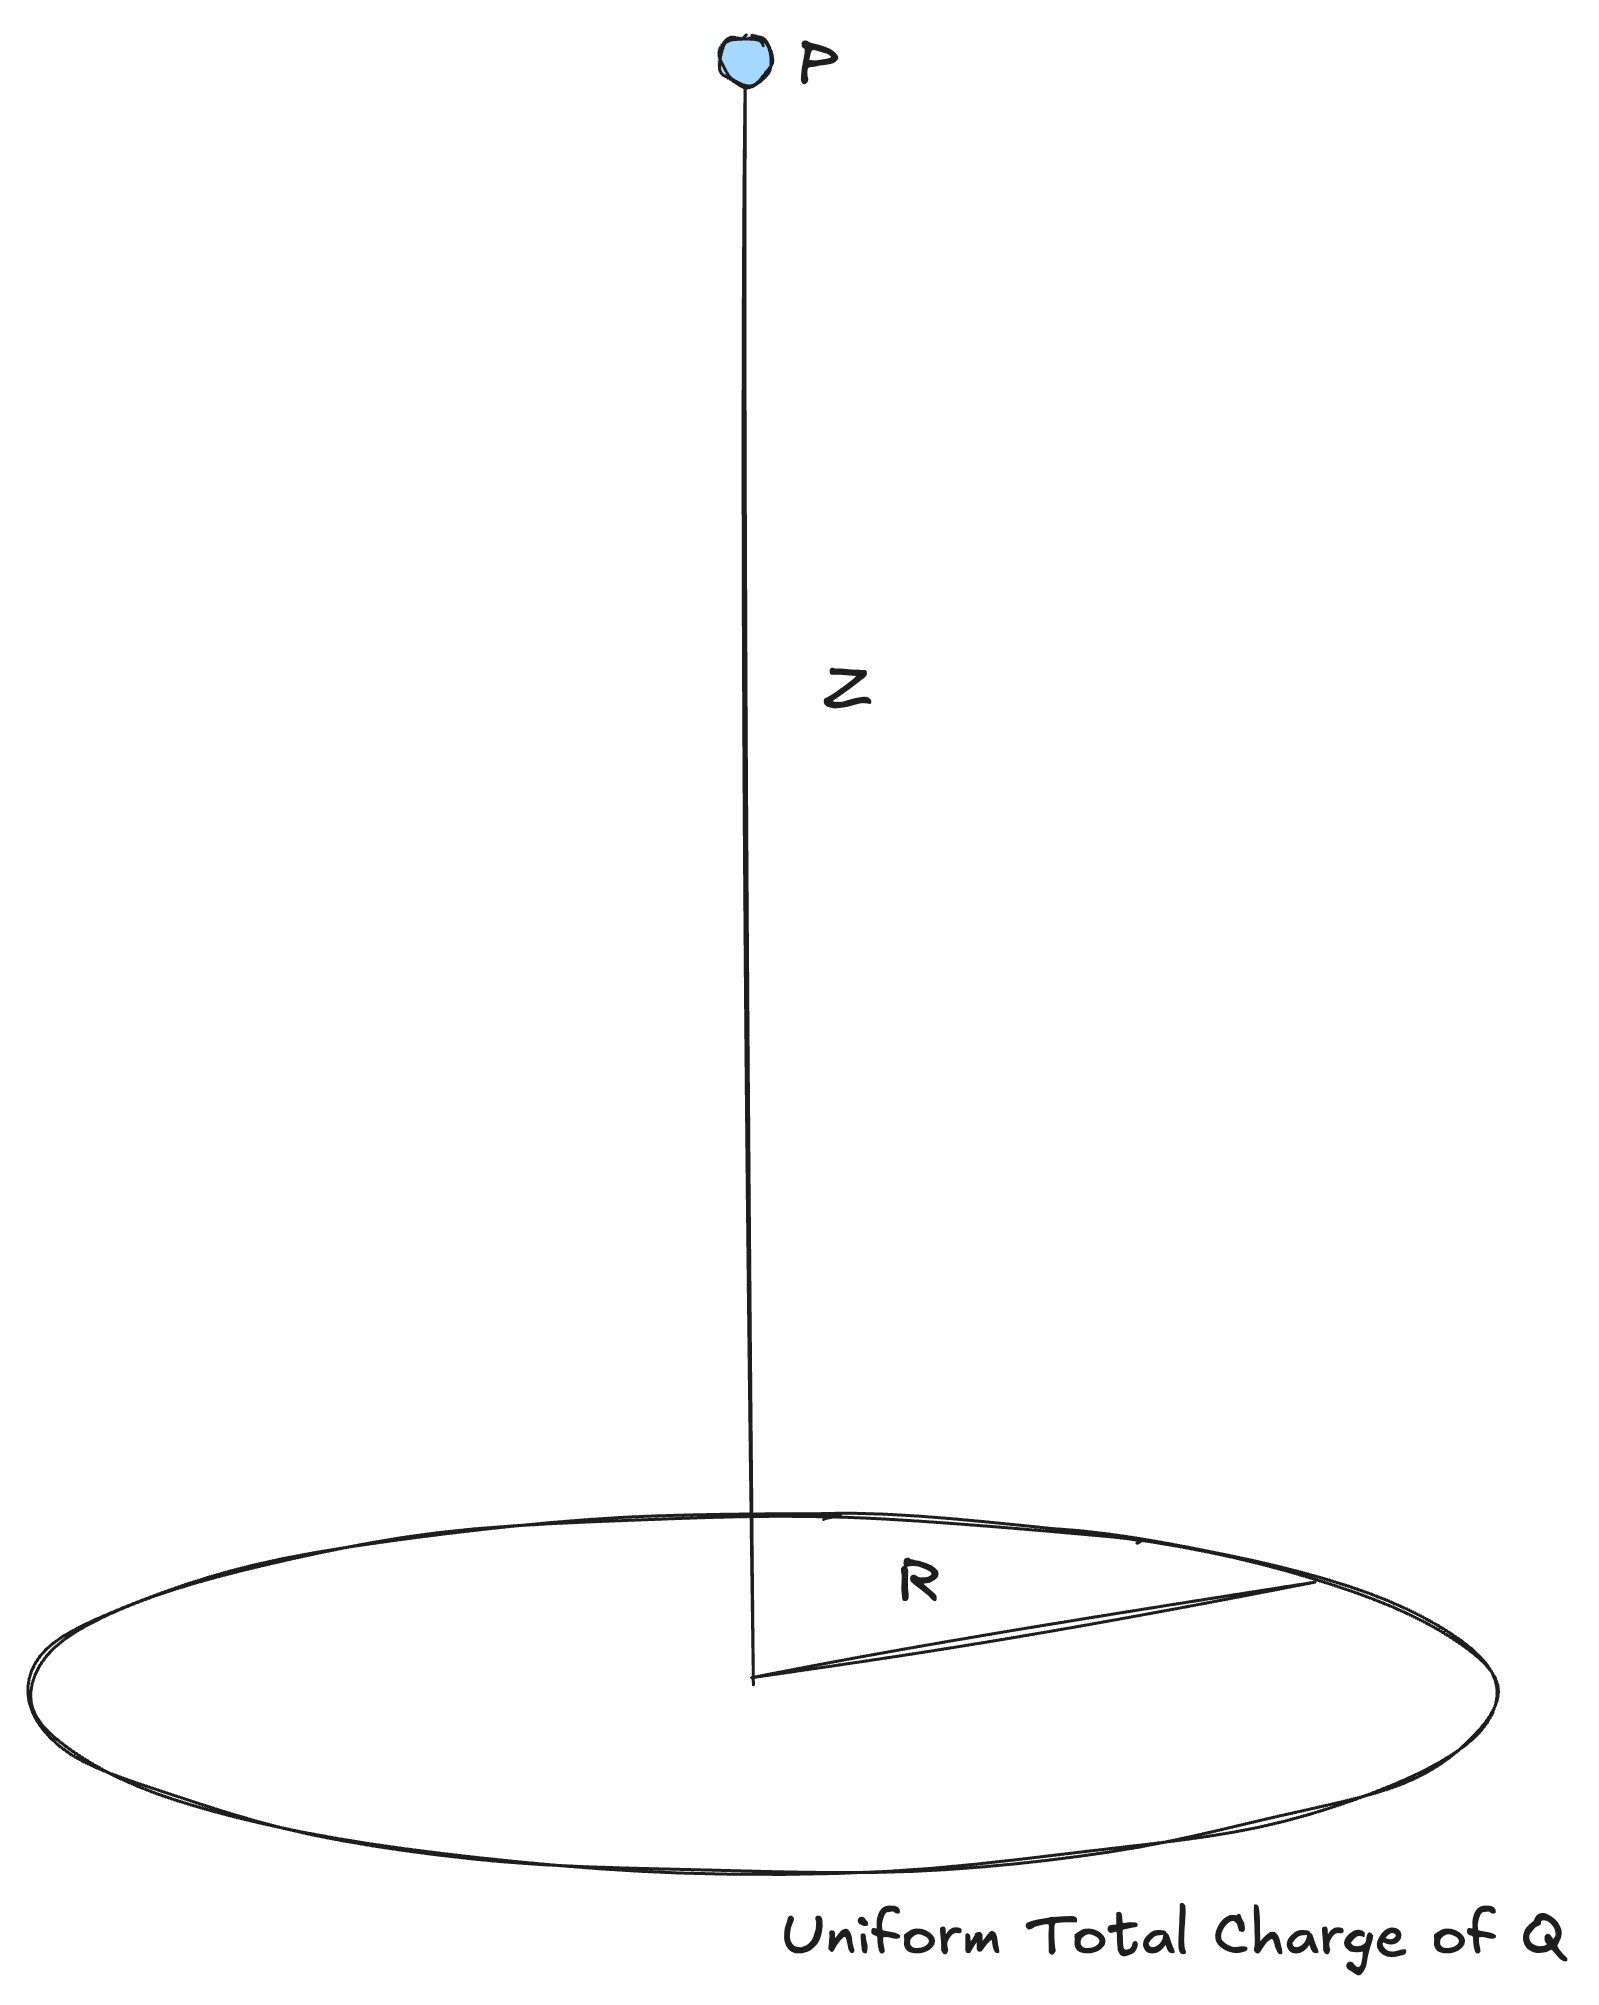
\includegraphics[width=0.3\textwidth]{figures/TheRing1.png}
    \caption{the Ring in question}
\end{figure}
Simplifications (it's a continious distance, but):
\begin{itemize}
    \item Symmetry
    \item Rigid Structure
\end{itemize}

\subsection{Deriving the Formula for Calculating the Electrical field}
Let's divide this method into several steps
\begin{enumerate}
    \item Define Charge Density
    \item Use symmetry
    \item Integration
\end{enumerate}

\textbf{\emph{Step 1}: Defining Charge Density}\\
Let's create a new value, and let's define it as charge density, $\lambda$, to help make this easier.

$$\lambda = \frac{\delta q}{\delta l} $$
Also, from the special case of it being a ring, we know that charge density is also the total charge minus the radius of the ring:
$$\text{Charge Density} = \frac{Q}{2 \pi r}$$
Then, we know that:
$$\lambda = \frac{\delta q}{\delta l} = \frac{Q}{2\pi r}$$
$$\delta q = \lambda \delta l$$

\textbf{\emph{Step 2}: Finding $\delta \vec{E}$ from $\delta q$ }\\
Let's first start with integrating and then substituting for the change in charge.
$$\delta \vec{E} = \frac{1}{4 \pi \epsilon R^2} \delta Q = \frac{1}{4\pi\epsilon} \frac{\lambda\delta l}{z^2 + r^2}$$
The visualization of the new figure:
\begin{figure}[H]
    \centering
    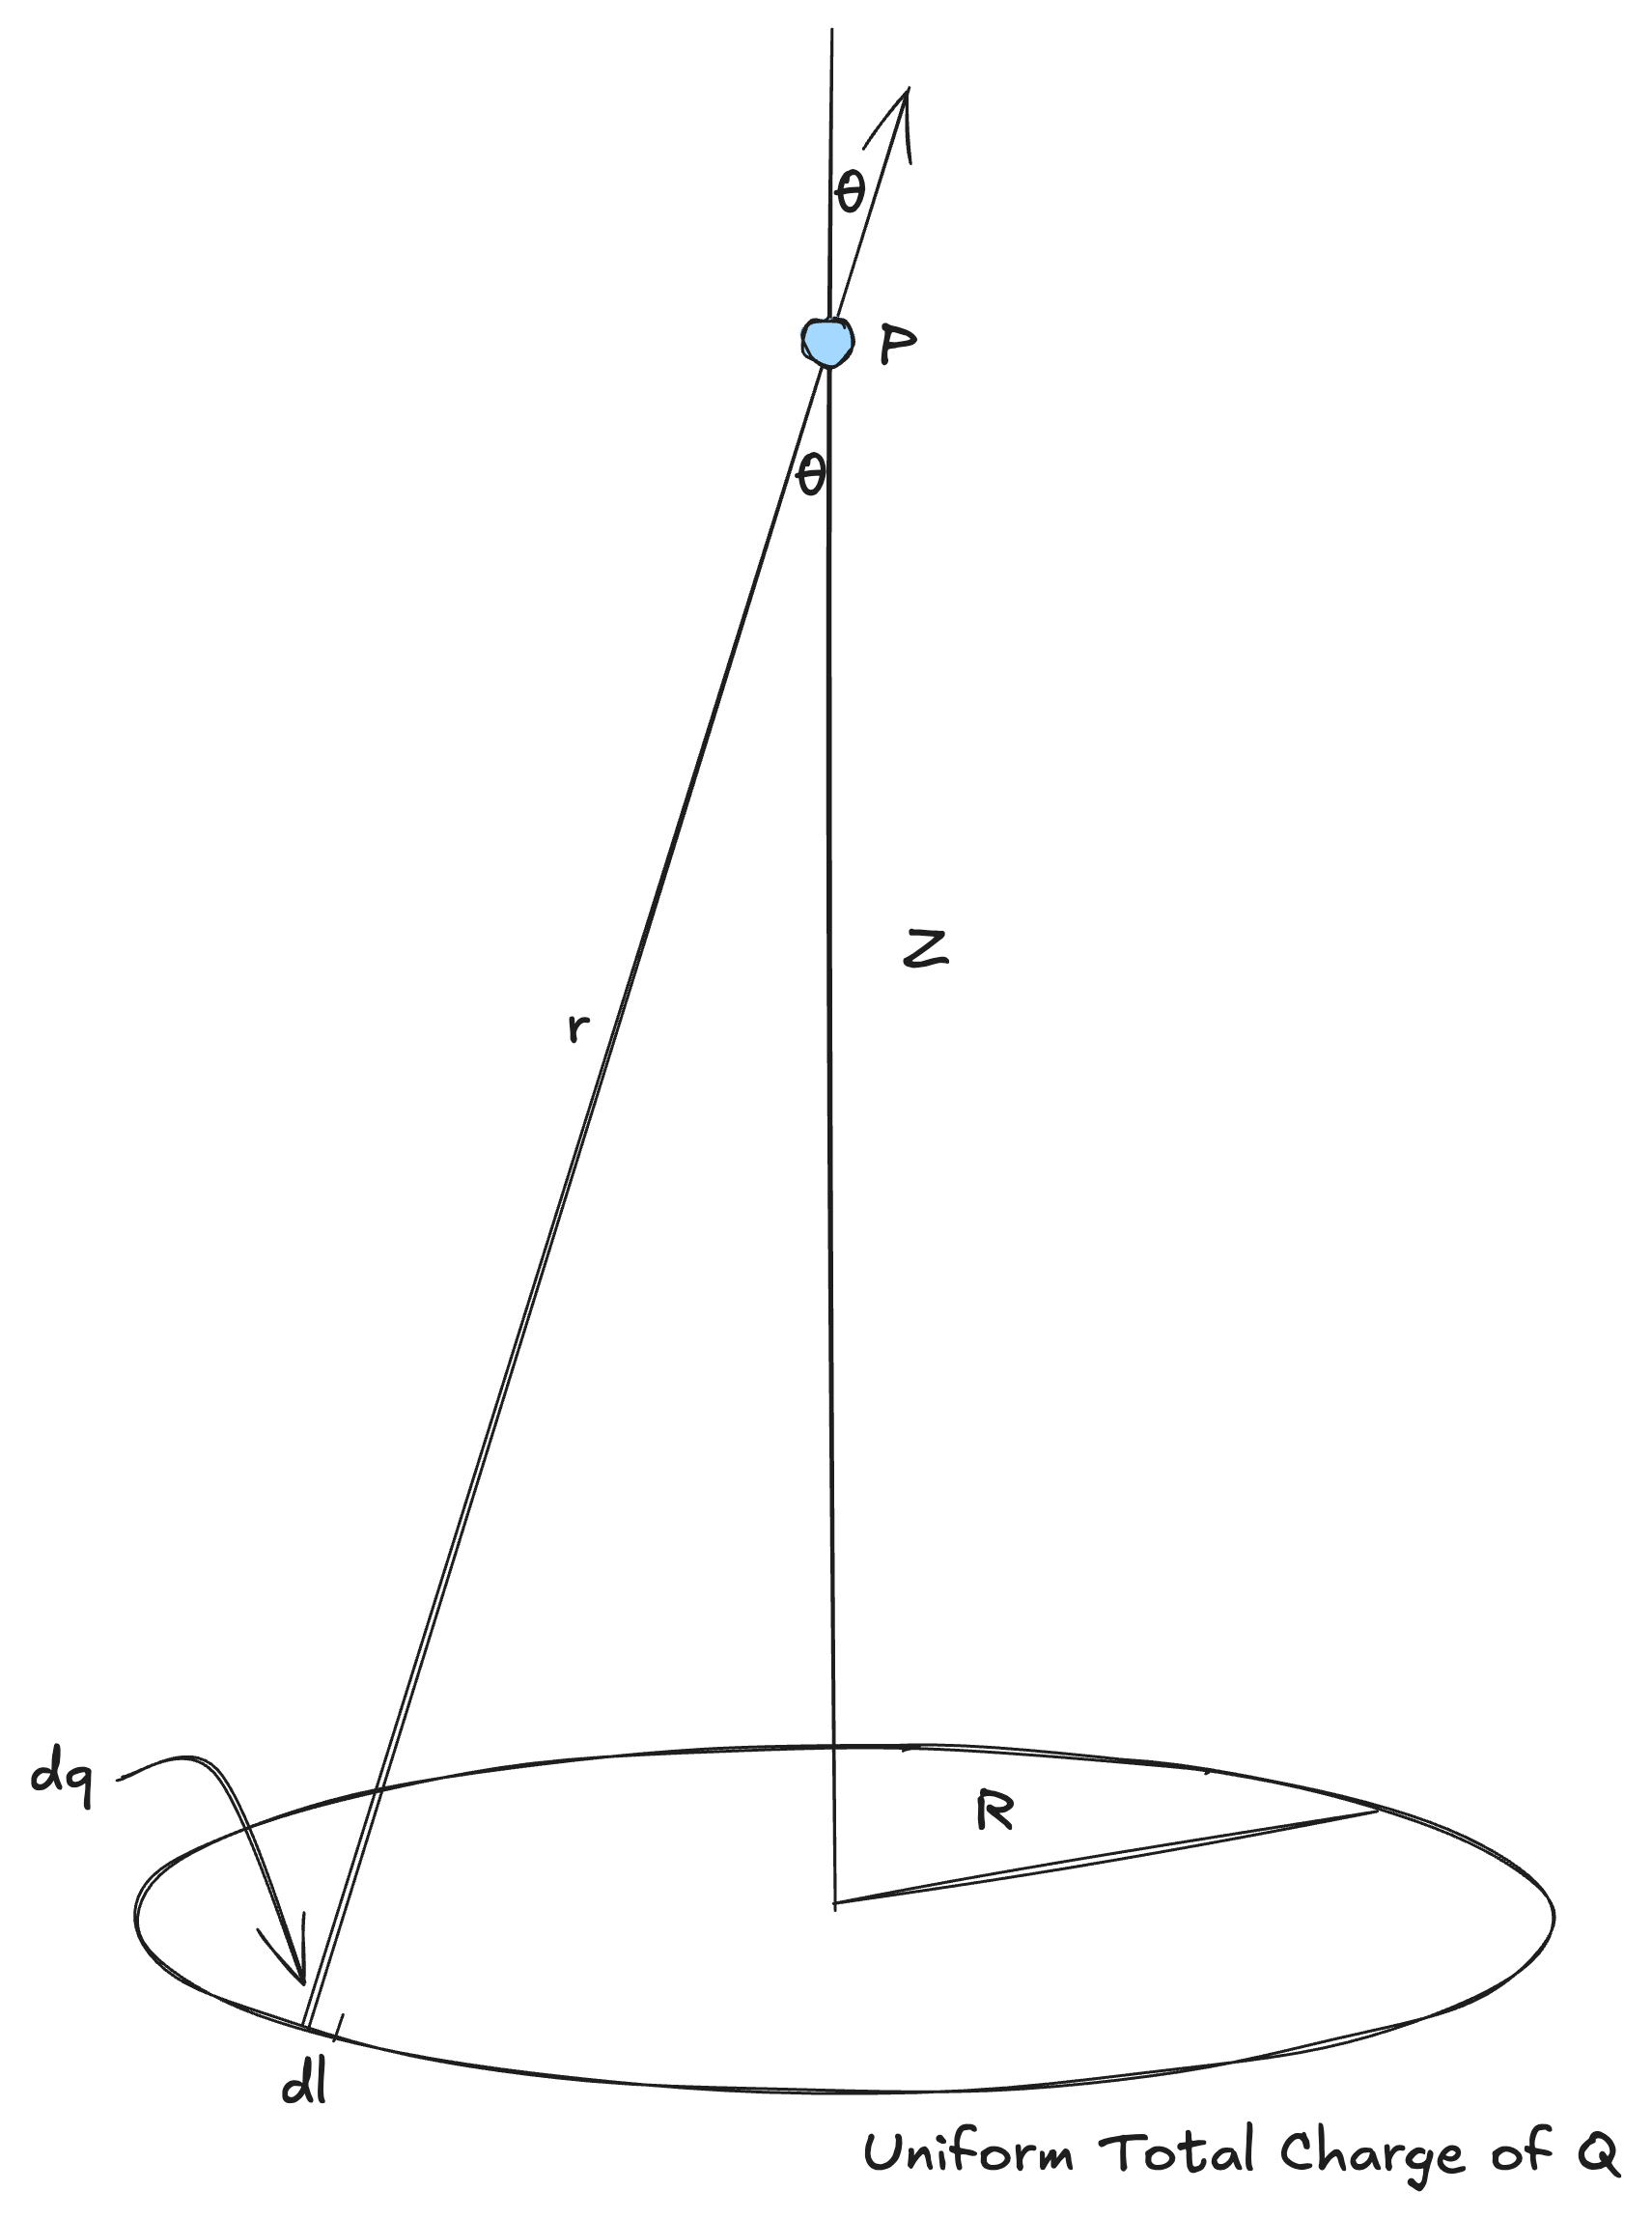
\includegraphics[width=0.3\textwidth]{figures/TheRing2.png}
    \caption{the Ring in question}
\end{figure}


\textbf{\emph{Step 3}: Use Symmetry}\\
\emph{Common sense time}: if you have two little $\delta \vec{F}$ from two little $\delta q$ from two $\delta l$ which are on opposite sides of circle, they cancel out. This is where we get $\delta \vec{E}_{\text{VERT}}$. After we integrate that, we should do some substituting
$$\delta E_{\text{VERT}} = \big| \delta \vec{E} \big| \cos \theta = \frac{1}{4\pi\epsilon} \frac{\lambda \delta l}{(z^2 + R^2)} \cos \theta$$
$$= \frac{1}{4\pi\epsilon} \frac{\lambda \delta l}{(z^2 + R^2)} \times \frac{z}{r}  \left[\cos(\theta) = \frac{z}{r} \right]$$
$$= \frac{1}{4 \pi \epsilon} \frac{\lambda \delta l}{(z^2 + R^2)^{3/2}} z$$
What's so great about this is that everything is constant, so integrating over the length of the ring would be trivial.


\textbf{\emph{Step 4}: Integrate}
$$\vec{E} = \int \delta E_{\text{VERT}} = \frac{1}{4 \pi\epsilon} \frac{\lambda z}{(z^2 + R^2)^{3/2}} \int_{0}^{2\pi R} \delta l$$
$$= \frac{\frac{Q}{2\pi R } z}{4 \pi \epsilon (z^2 + R^2)} 2\pi R   \left[ \text{\textbf{NOTE}: } \lambda = \frac{Q}{2 \pi R} \right]$$
$$= \boxed{\frac{Qz}{4\pi\epsilon(z^2 + R^2)^{3/2}}}$$

\textbf{Some Test Cases}
\begin{itemize}
    \item $E_{z = 0} = 0$
    \item $E_{z >> r} = \frac{Q}{4\pi\epsilon z^2}$ [basically the point formula, its very far away it behaves like a point particle]
\end{itemize}

\section{Calculating Continuous Charge Distributions for a Charged Circular Rod}

To solve this problem, let's do a few things:

\begin{itemize}
    \item Define Linear Charge Density, $\lambda$
    \item Pick infintesimal charge element and define the infintesimal field from the infintesimal charge
    \item Use Symmetry to determine the component that wouldn't cancel
    \item Change variables as needed and integrate to find the field
\end{itemize}

\begin{figure}[H]
    \centering
    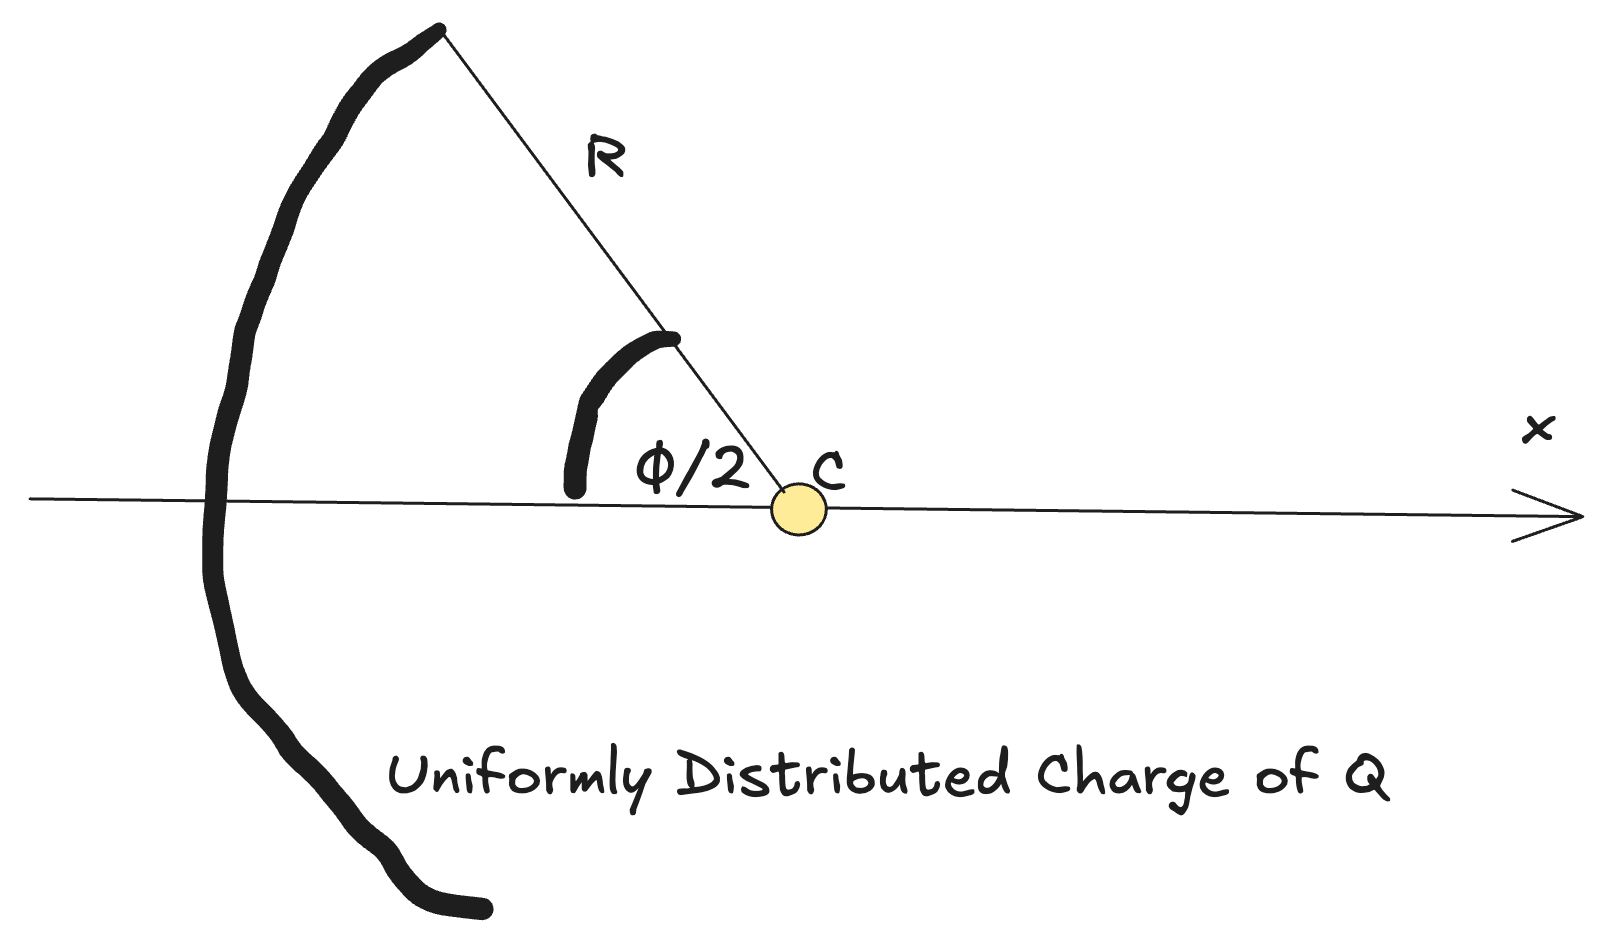
\includegraphics[width=0.5\textwidth]{figures/ChargedCircularRod.png}
    \caption{Example of a charged circular rod}
\end{figure}

\textbf{\emph{Step 1}: Defining Linear Charge Density}\\
Let's try to find $\lambda$ and its relations to angle
$$\lambda= \frac{\delta Q}{\delta L} = \frac{Q}{2\pi r \frac{\phi}{2\pi}} = \frac{Q}{\phi R}$$
$$\delta Q = \lambda \delta l$$
$$\delta L = R \delta \theta$$
$$\delta Q = R \lambda \delta Q$$

\textbf{\emph{Step 2}: Defining the Infintesimal Field from the Infintesimal Charge}
$$\delta \vec{E} = \frac{1}{4 \pi\epsilon R^2} \delta Q = \frac{1}{4\pi\epsilon} \frac{Q}{\phi R} \delta l$$

\textbf{\emph{Step 3}: Use Symmetry to Uncancelable Component}

$$\delta \vec{E}_{\text{NC}}  = \delta \vec{E} \cos(\theta) = \frac{1}{4\pi\epsilon}\frac{Q}{\phi R} \cos(\theta) \delta l $$

\textbf{\emph{Step 4}: Change Variables and Integrate}

$$\delta \vec{E}_{\text{NC}} = \frac{1}{4\pi\epsilon R^2} \frac{Q}{\phi R} \cos(\theta) \delta l = 1\frac{1}{4\pi\epsilon R^2} \cos(\theta) \frac{Q}{\phi R} R \delta \theta$$
$$\vec{E} = 2 \int_{0}^{\frac{\phi}{2}} \frac{1}{4\pi\epsilon R^2} \frac{Q}{\phi R} R \cos(\theta) \delta \theta$$
$$= \boxed{\frac{Q}{4\pi\epsilon R^2 \phi} 2 \sin\left(\frac{\phi}{2}\right)}$$

\section{Find the Electrical Field of a Disk}
Find the electrical field of a point a distance z above a uniformly charged disk of radius R, with area A.

\begin{figure}[H]
    \centering
    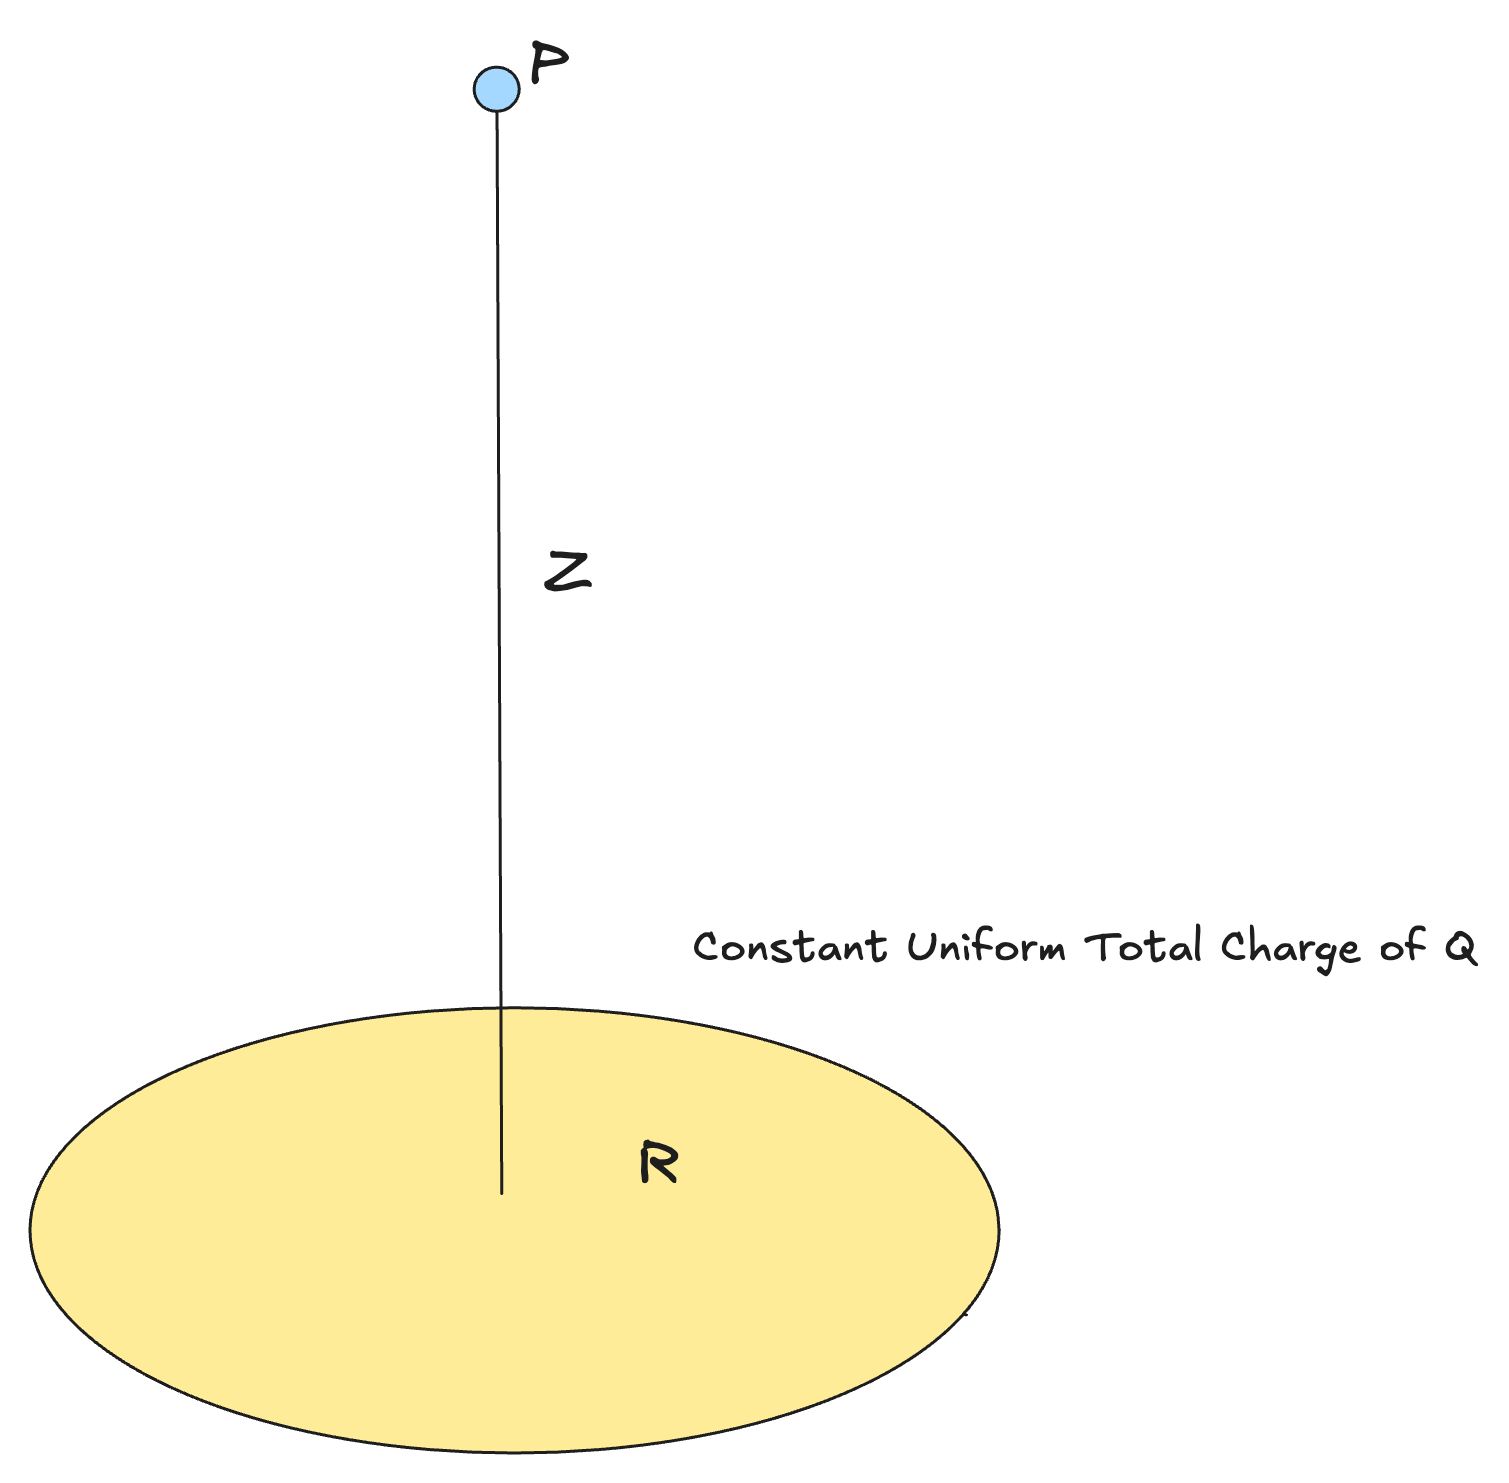
\includegraphics[width=0.5\textwidth]{figures/DiskCharged.png}
    \caption{Example of a charged disk}
\end{figure}

\textbf{\emph{Step 1}: Find charge density}\\
$\sigma$ is the charge density

$$\sigma = \frac{\delta q}{\delta A} = \frac{Q}{\pi R^2}$$
$$\delta q = \sigma \delta A$$

Let's now split the disk into rings of radius $r (0 < r < R)$, thickness $\delta r$ and charge $\delta q = \sigma \delta A$
$$\delta A = 2 \pi r \delta r$$
$$\delta q = \sigma \delta A = 2 \pi r \sigma \delta r$$

\textbf{\emph{Step 2}: Finding an infintesimal field from infintesimal charge}

$$\delta \vec{E} = \frac{z \delta q}{4 \pi \epsilon (z^2 + r^2) ^{\frac{3}{2}}} = \frac{z \sigma }{4 \epsilon} \frac{2r\delta r}{(z^2 + r^2) ^ {\frac{3}{2}}}$$

\textbf{\emph{Step 3}: Integrate}
$$\text{Let } u = z^2 + r^2; \delta u = 2r\delta r$$
$$\vec{E} = \frac{z \sigma}{ 4 \epsilon} \int_{0}^{R} \frac{zr}{(z^2 + r^2)^{\frac{3}{2}}} \delta r$$
$$= \frac{z \sigma}{4 \epsilon} \int_{z^2}^{z^2 + r^2} u ^{-\frac{3}{2}} \delta u = -\frac{z \sigma}{4 \epsilon} \left|u^{-\frac{1}{2}}\right|_{z^2}^{z^2 + r^2}$$
$$= - \frac{z \sigma}{4 \epsilon}\left[\frac{1}{\sqrt{z^2 + k^2}}- \frac{1}{z}\right] = \frac{z \sigma}{4 \epsilon}\left[\frac{1}{z} - \frac{1}{\sqrt{z^2 + k^2}}\right]$$
$$= \frac{\sigma}{2 \epsilon} \left[1 - \frac{z}{\sqrt{z^2 + r^2}}\right] = \boxed{\frac{Q}{2 \pi R^2  \epsilon} \left[1 - \frac{z}{\sqrt{z^2 + r^2}}\right]}$$

\textbf{Some Checks} \
Just some limits tomfoolery

$$E\left(^{z \to\infty}_{R\to\infty}\right) = \frac{\sigma}{2 \epsilon}$$


\section{Constant Electric Field}
Constant electric fields are just that. They're constant, and they apply to particles in interesting ways, very similar to gravity.
\begin{figure}[H]
    \centering
    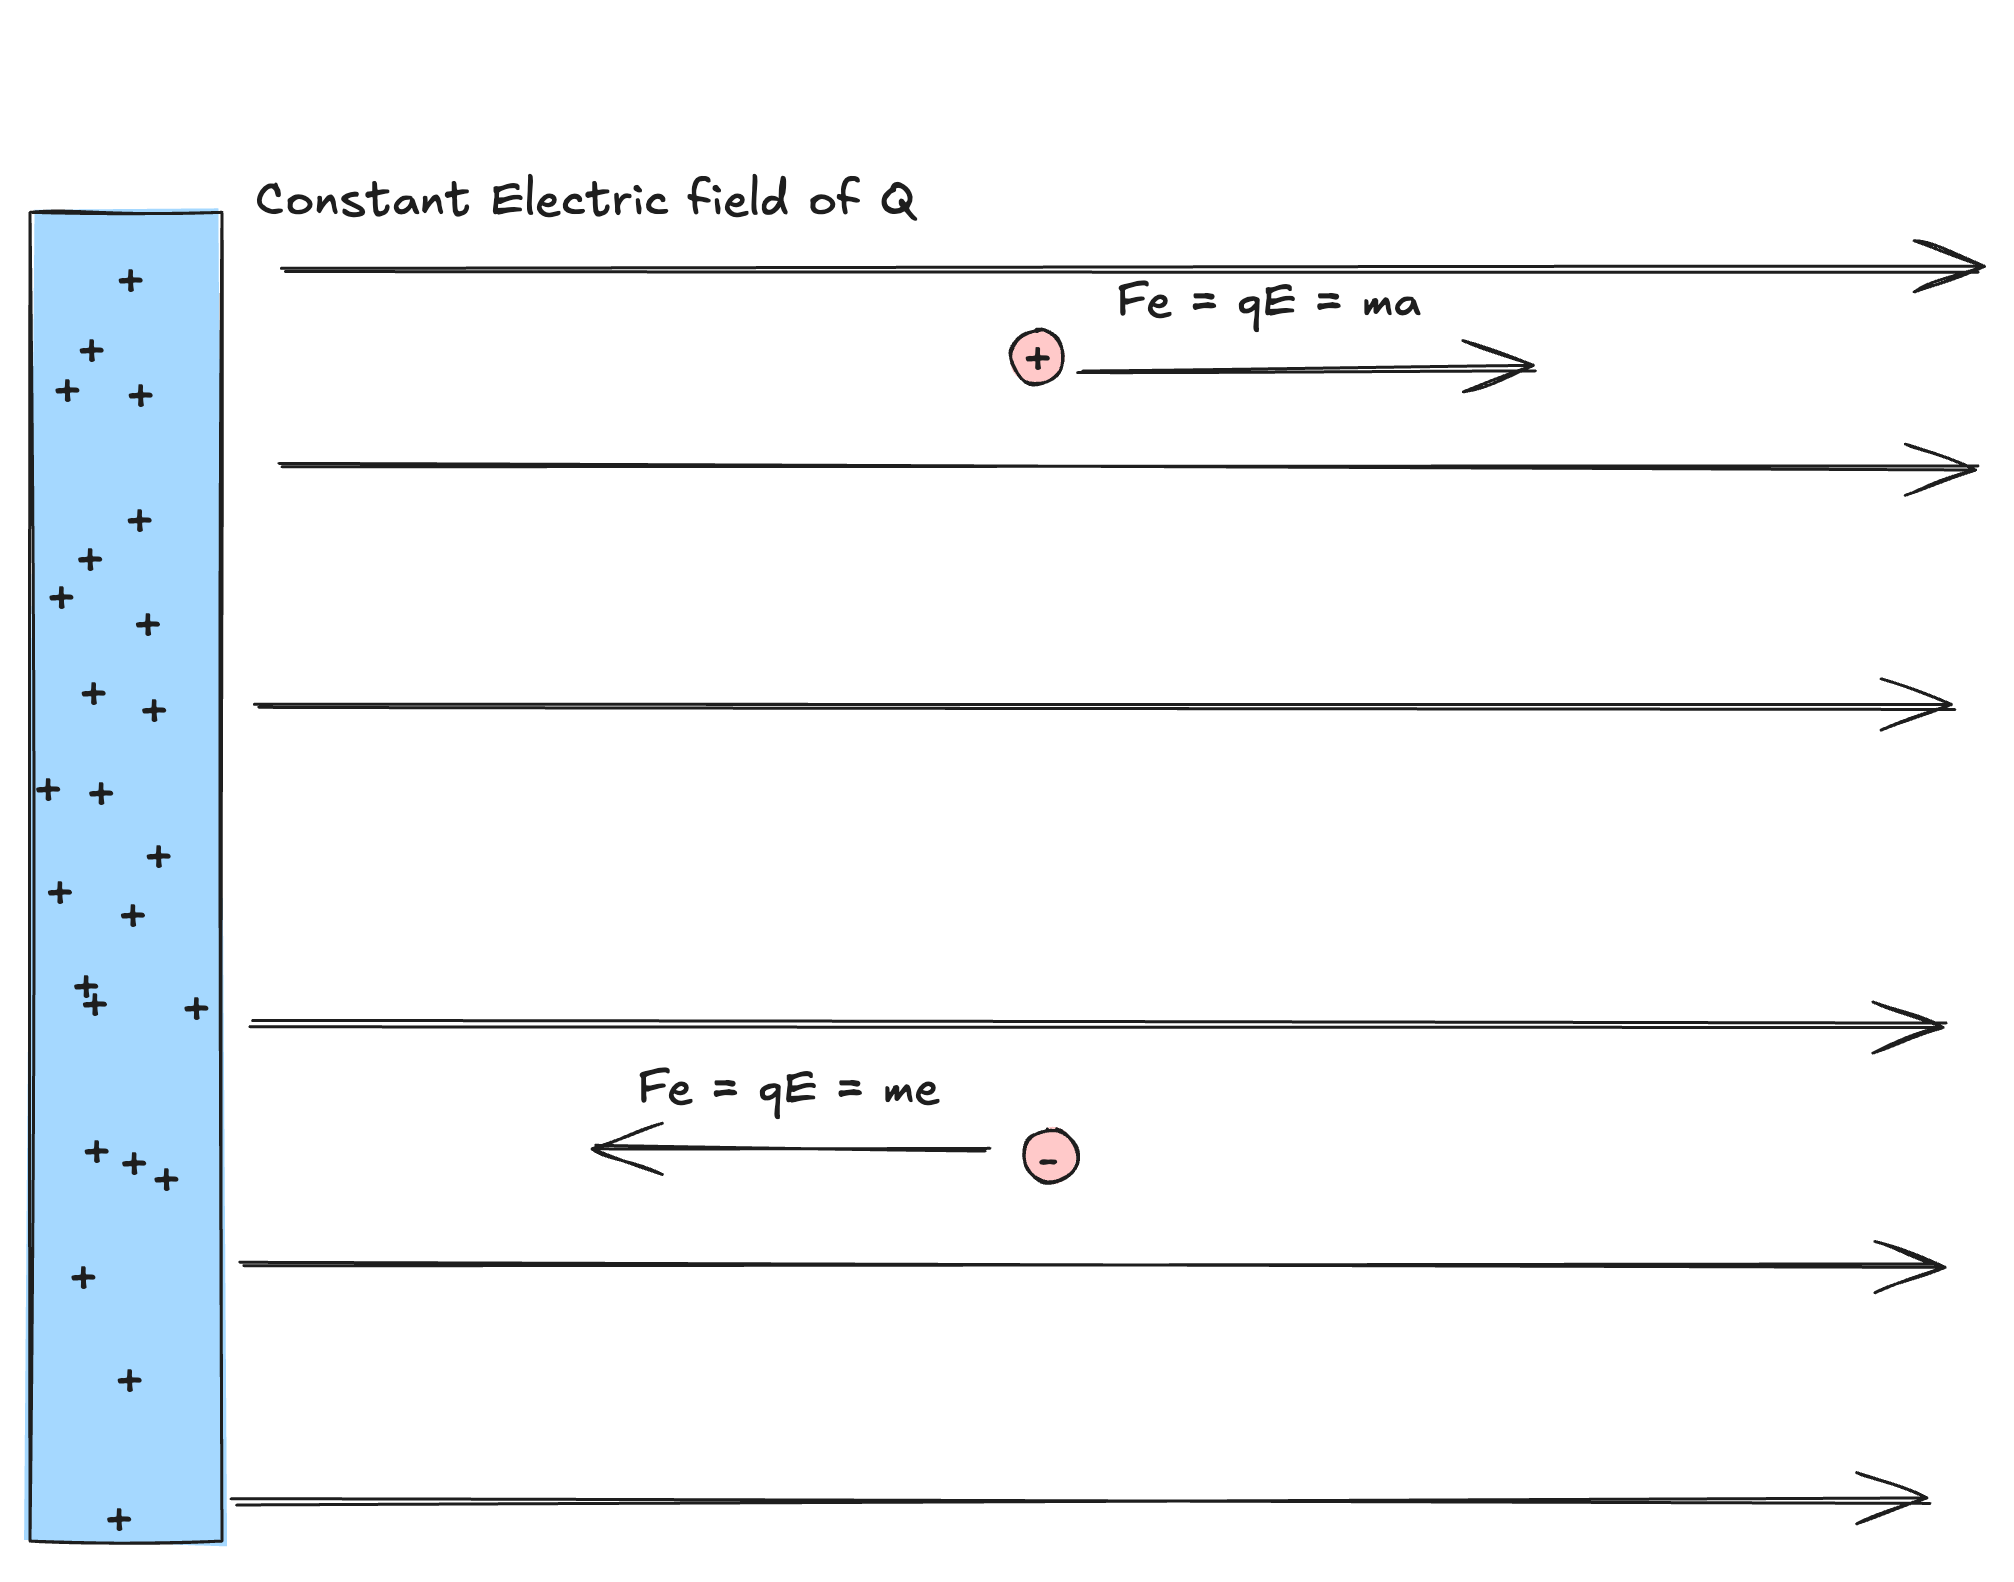
\includegraphics[width=0.5\textwidth]{figures/ConstantElectricFieldIntro.png}
    \caption{Example of a constant electric field }
\end{figure}

You get parabolic stuff too, if apply an initial velocity.

\begin{figure}[H]
    \centering
    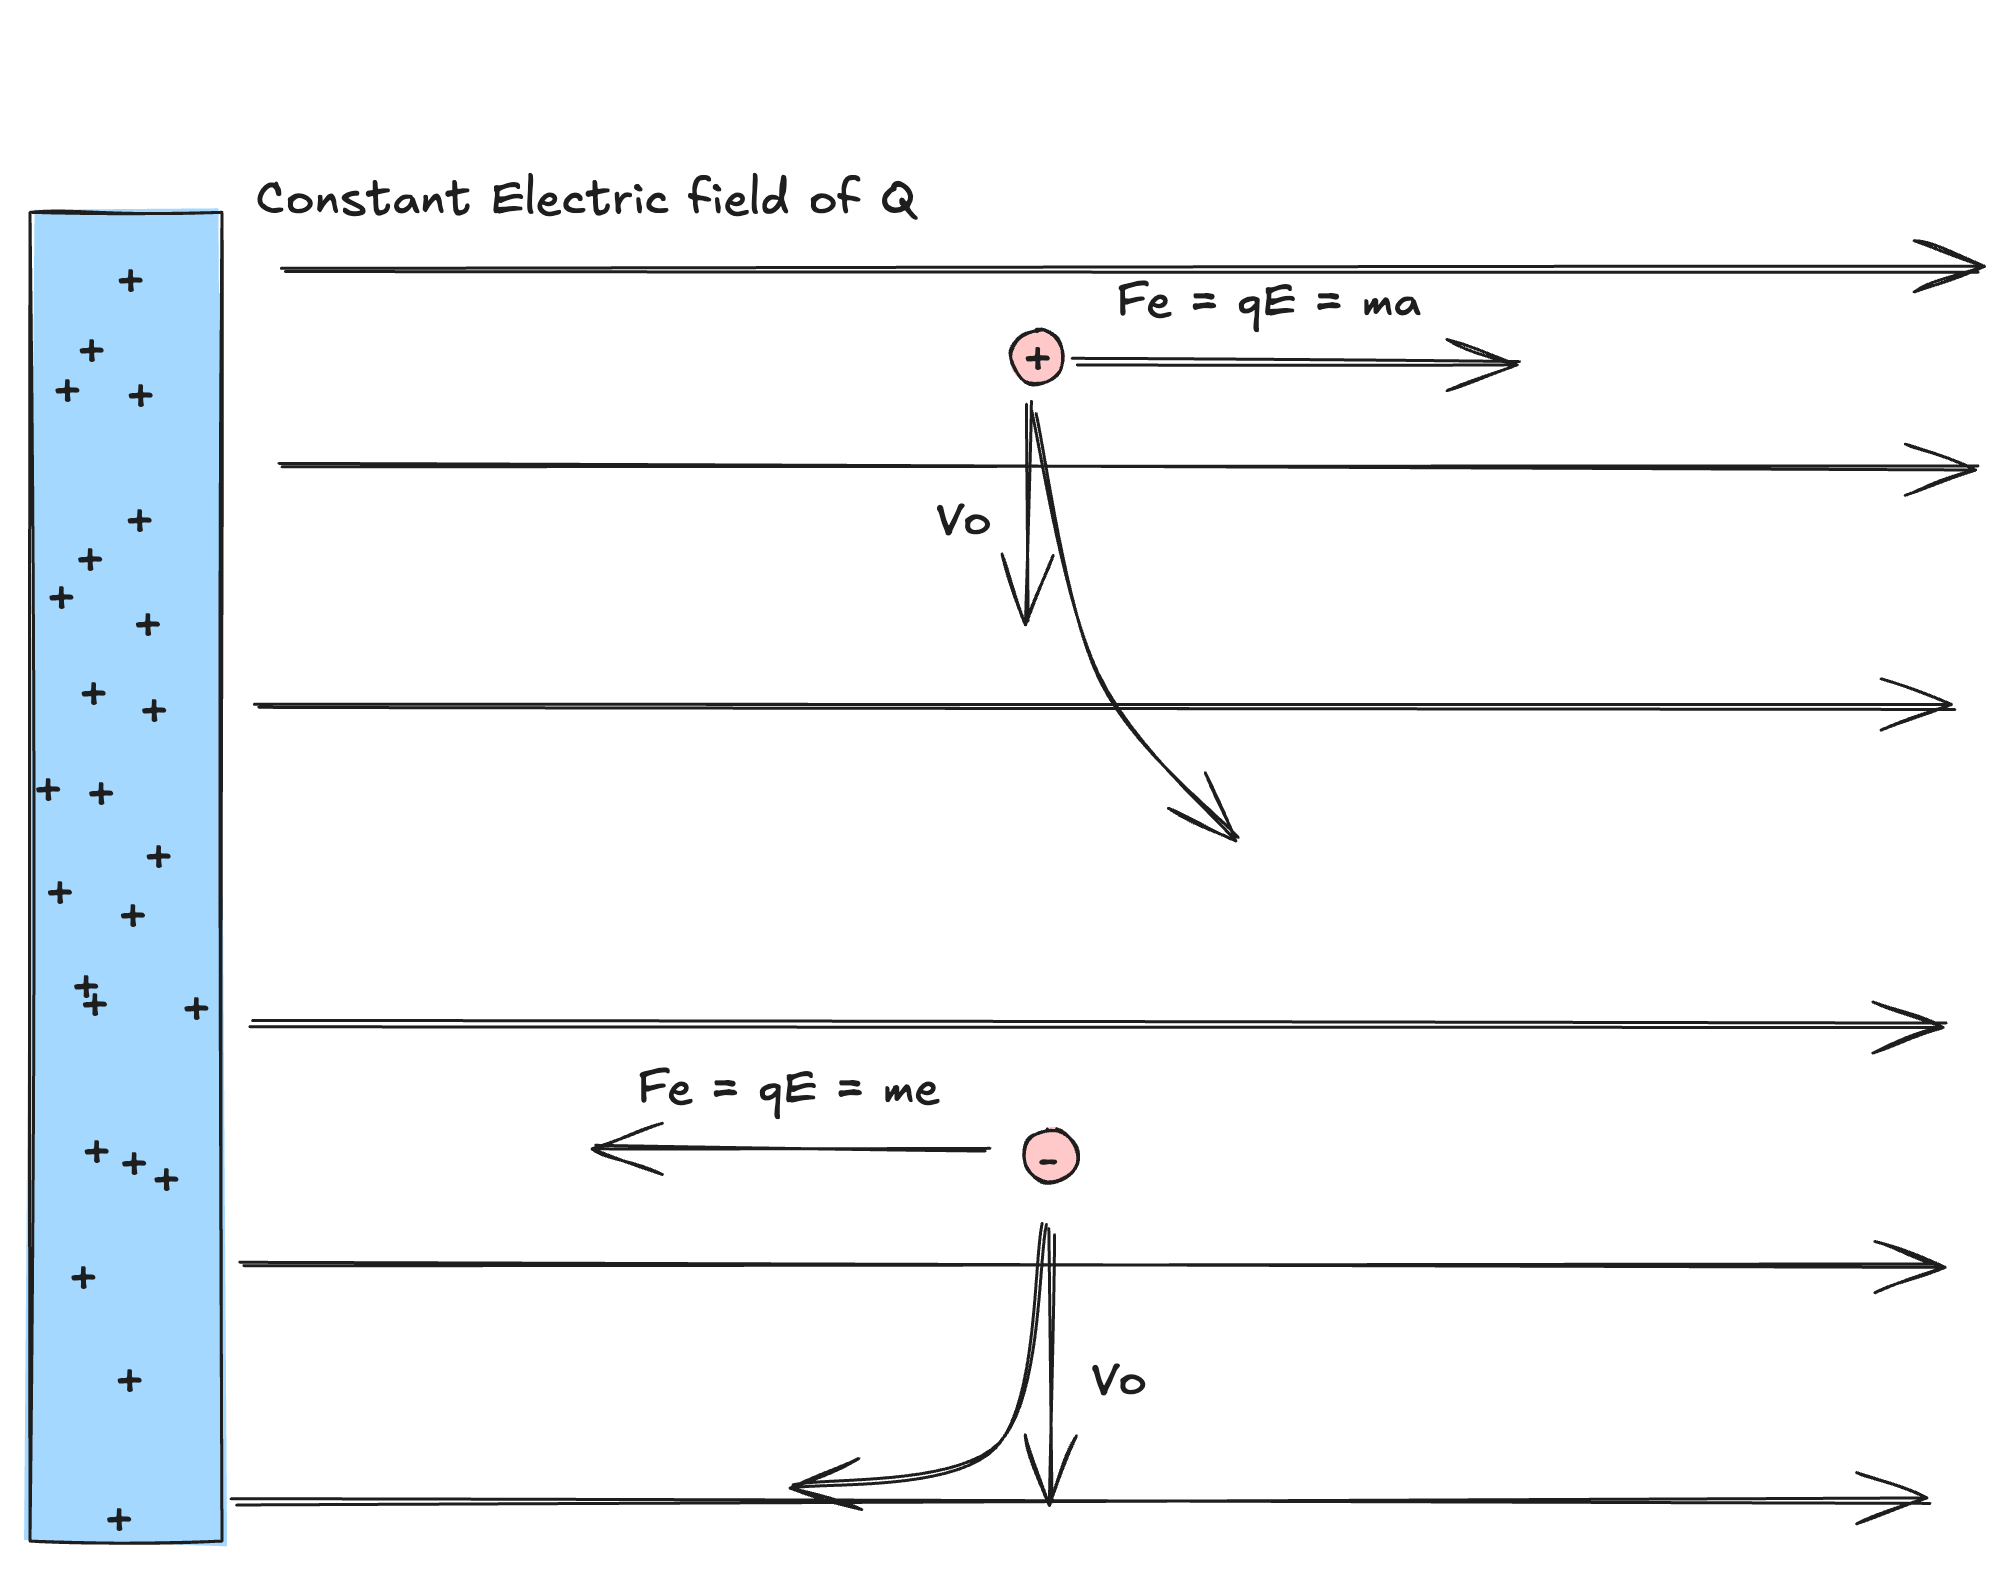
\includegraphics[width=0.5\textwidth]{figures/ConstantFieldsWithInitialVs.png}
    \caption{Example of a constant electric field with an initial velocity}
\end{figure}

\section{Electrical Potentials}
Electric potentials are measures of the potential energy created by an electric field.
You can think of them as such:

\begin{center}
    Potential: Potential Energy :: Field: Force Energy
\end{center}
For the potential energy of point charges, there is a very big positional element here. As long as you have two charged particles, as long as they want to move somewhere, there will always be potential energy in that system. Usually, systems want to reduce that energy to zero.

\subsection{Formulas and Dimensional Analysis}
Let's look at the formulas for volts and field, and see what we can make for them. Let's have the formula for volts, and put of the formula for electric field for comparison.

\begin{align*}
    V = \frac{U}{q} &  & \vec{E} =  \frac{\vec{F}}{q}
\end{align*}

Let's do a quick dimensional analysis too for these \emph{volts}:

$$[V] = \frac{[J]}{[C]}$$

Differences between field and potential:

\begin{itemize}
    \item Field is a vector quantity, voltage is a scalar quantity
    \item Field lines are always perpendicular accross vector lines
\end{itemize}

Let's have a visualization changes of potential over time:

\begin{figure}[H]
    \centering
    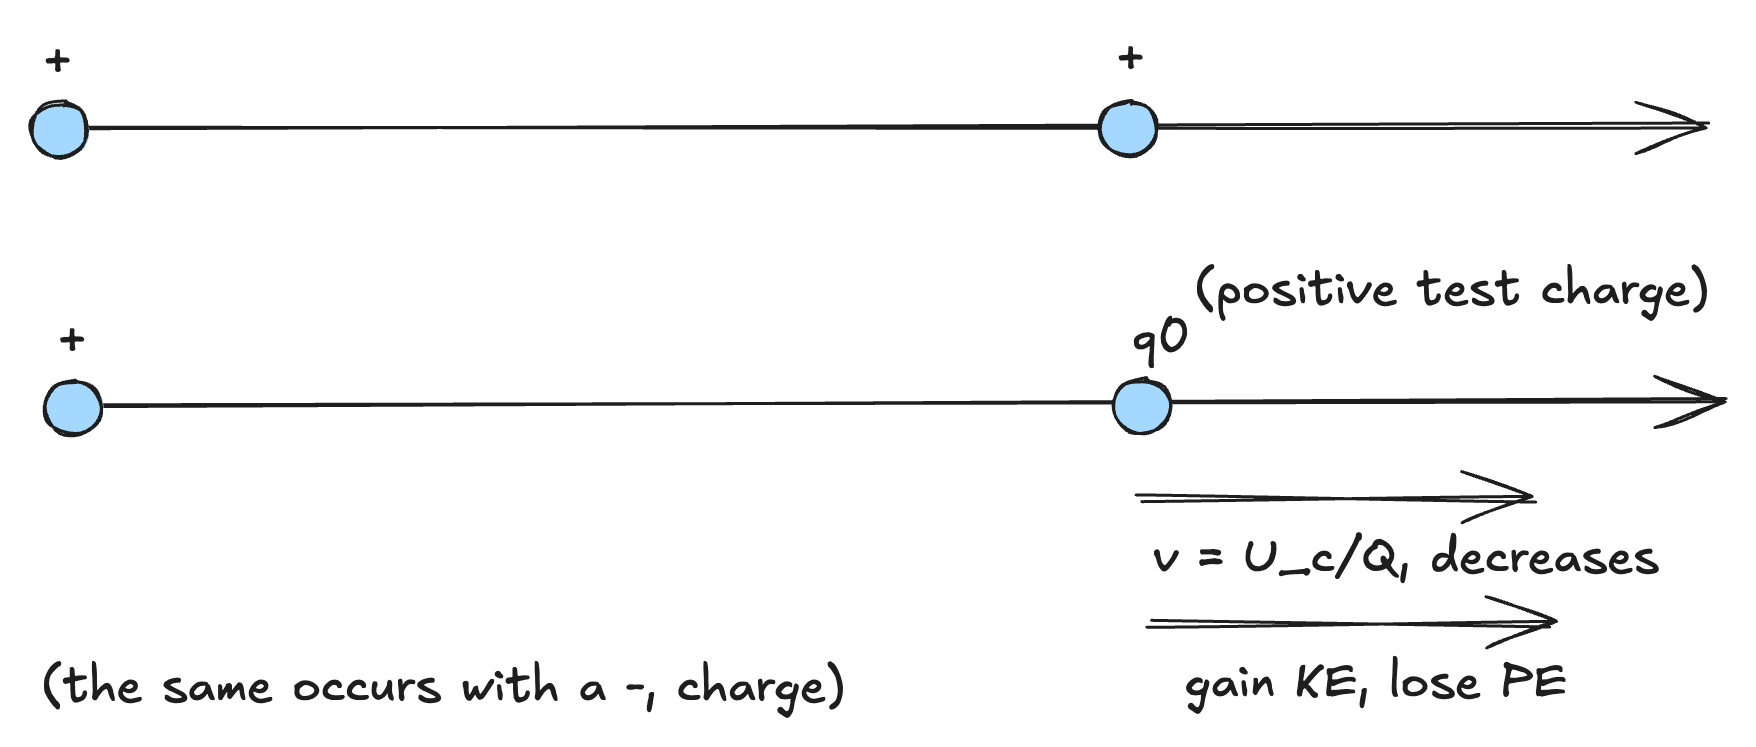
\includegraphics[width=0.5\textwidth]{figures/ChangeVAccrossNumberLine.png}
    \caption{The change of charge accross a number line}
\end{figure}

Notes:
\begin{itemize}
    \item Voltage decreases as one goes through a field lines
\end{itemize}

\subsection{Equipotentials}

\begin{figure}[H]
    \centering
    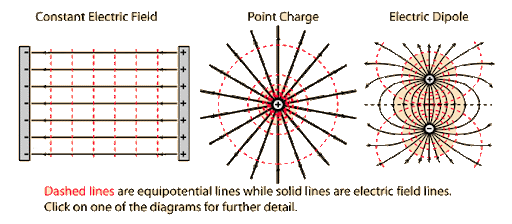
\includegraphics[width=0.5\textwidth]{figures/FieldvsPotentials.png}
    \caption{Example of electric fields vs electric potentials}
\end{figure}

\begin{itemize}
    \item Lines accross these show the areas of equidistant potentials
    \item Circular around point charge
    \item \emph{Perpendicular to field lines}, (e.g. Electric field is the negative gradient of potential), or $E = - \Delta V$
\end{itemize}

\subsection{Calculating Electrical Potential from Electric Field}
\begin{figure}[H]
    \centering
    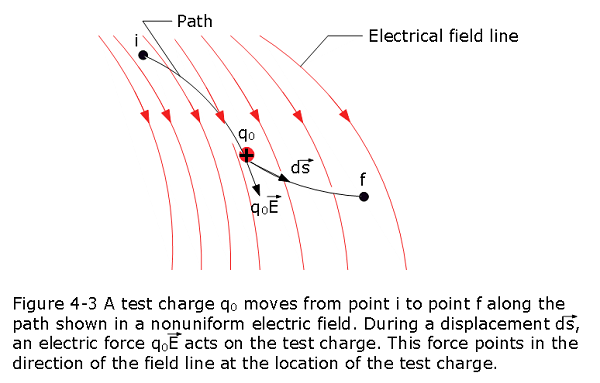
\includegraphics[width=0.5\textwidth]{figures/PotentialChanges.png}
    \caption{Visualization of the different differentials here}
\end{figure}

To try to find a formula for this, starting from the givens and working up.

\begin{align*}
    \vec{F} = q_0 \vec{E} &  & W = \int \delta W
\end{align*}

$$W = \int \delta w =  \int_{i}^{f} \vec{F} \delta \vec{s}$$
$$ = - \Delta U = - q_0 \Delta V $$
$$ \Delta v = \boxed{-\int_{i}^{f} \vec{E} \delta s}$$

Given that electric field is a vector, and potentials are scalars, one might have to treat these as partial derivatives of x and y. So we have the original equation:

$$\vec{E} = \frac{Q}{4 \pi \epsilon R^2} = - \frac{\delta V}{\delta s}$$

But we have to split it into components:

\begin{align*}
    E_x = \frac{\delta V}{\delta x} &  & E_y = \frac{\delta V}{ \delta y} \\
\end{align*}

$$  \vec{E} = - \frac{\Delta V}{\Delta S} = \frac{\delta V}{\delta x} + \frac{\delta V}{\delta y}$$



\end{document}

